\documentclass[tikz]{standalone}

\usetikzlibrary{calc,positioning,shapes,positioning,intersections,quotes,decorations.markings}
\usepackage{amsfonts,amsmath,amsthm,amssymb,mathtools,stmaryrd,mathrsfs}

\begin{document}
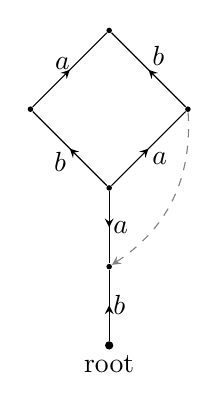
\begin{tikzpicture}[>=stealth,decoration={
				markings,
				mark=at position 0.5 with {\arrow{>}}}
	]

	\node[circle,fill=black,inner sep=0pt,minimum size=3pt] (m1) at (0,0){} node[below]{root};

	\node[circle,fill=black,inner sep=0pt,minimum size=2pt] (n0) at (0,1){};
	\node[circle,fill=black,inner sep=0pt,minimum size=2pt] (n1) at (0,2) {};
	\node[circle,fill=black,inner sep=0pt,minimum size=2pt] (n2) at (1,3) {};
	\node[circle,fill=black,inner sep=0pt,minimum size=2pt] (n3) at (0,4) {};
	\node[circle,fill=black,inner sep=0pt,minimum size=2pt] (n4) at (-1,3) {};

	\draw[postaction={decorate}] (m1) --node[right=-2pt]{$b$} (n0);
	\draw[postaction={decorate}] (n1) --node[right=-2pt]{$a$} (n0);
	\draw[postaction={decorate}] (n1) --node[below right=-3pt]{$a$} (n2);
	\draw[postaction={decorate}] (n2) --node[above right=-3pt]{$b$} (n3);
	\draw[postaction={decorate}] (n4) --node[above left=-5pt]{$a$} (n3);
	\draw[postaction={decorate}] (n1) --node[below left=-3pt]{$b$} (n4);


  \draw[->, dashed,gray] (n2) to[bend left] (n0);


\end{tikzpicture}
\end{document}
